\documentclass[12pt, a4paper, twocolumn]{article}

\newcommand{\getTitle}{Principles of Object-Oriented Programming Languages: Language Comparison}
\newcommand{\getAuthor}{Mathijs Saey}
\newcommand{\getFullTitle}{Principles of Object-Oriented Programming Languages: \\ Language Comparison}
\newcommand{\getFullAuthor}{Mathijs Saey, 94451,  \\ mathsaey@vub.ac.be, \\ 1st Master of Science in Applied Sciences and Engineering: \\ Computer Science}

\newcommand{\mytilde}{\raise.17ex\hbox{$\scriptstyle\mathtt{\sim}$}}

%Packages
\usepackage{color}
\usepackage{graphicx} 
\usepackage{listings}
\usepackage{longtable}

%Bibliography
\usepackage{biblatex}
\addbibresource{references.bib}

%Hyperref + pdf meta info
\usepackage[hidelinks]{hyperref}

\hypersetup{
 	pdfauthor={\getAuthor},
 	pdftitle={\getTitle},
 	pdfkeywords={VUB, Object-oriented, C++, Objective-C},
 	pdfproducer=pdfLatex,
 	pdfcreator=Sublime Text 2,
}

%Extra colors
\definecolor{dkgreen}{rgb}{0,0.6,0}
\definecolor{gray}{rgb}{0.9,0.9,0.9}
\definecolor{mauve}{rgb}{0.58,0,0.82}

% Listing settings
\lstset{language=C++,
	basicstyle=\scriptsize,
	backgroundcolor=\color{gray},
	commentstyle=\color{dkgreen},
	numberstyle=\scriptsize\color{black},
	keywordstyle=\color{blue},
	morekeywords={@interface, @end, @protocol, @implementation, alloc, init, import, id},
	numbers=left,
	xleftmargin=9pt,
	framexleftmargin=9pt,
	breaklines=true,
	numbersep=1pt,
	tabsize=2}


\begin{document}

%Options
\setlength{\parindent}{0pt}
\setlength{\parskip}{1ex}

%Title + table of contents
\onecolumn 
%Title page
\title{\getTitle}
\author{\getFullAuthor}
\date{\today}
\maketitle

%Vub Logo
\begin{figure}[!]
\centerline{

\includegraphics[scale=0.2]{files/vub_logo.jpg}}
\end{figure}
\newpage
\tableofcontents
%Content

\section{Introduction}
\subsection{About}
This paper is written for the Principles of Object Oriented Languages course at the VUB. The goal of this paper is to compare the object-oriented properties of 2 languages. 

\subsection{Languages}
Objective-C and C++ were chosen for this purpose, these languages are both strict supersets of C, but have a very different approach on object oriented features. C++ is focussed towards run-time efficiency and static type checking \cite{CPdesc}; while Objective-C tries to do things dynamically whenever this is possible \cite{OCRPG}.

Both languages were compiled with llvm-gcc, with the following version info: "i686-apple-darwin11-llvm-gcc-4.2 (GCC) 4.2.1 (Based on Apple Inc. build 5658) (LLVM build 2336.11.00)". In the case of Objective-C, the \textit{Foundation} runtime was used (received by appending -framework Foundation to the standard gcc compile instruction). Finally, all of the code files and their respective makefiles can be found at \url{https://github.com/mathsaey/POOL-Paper} in case of any issues.

\subsection{Structure}
At first, the general properties of both languages will be compared (such as access levels and the typing system). Afterwards, we will discuss the language features that are unique to each language and attempt to explain their absence in the other language.

\section{General properties}
\label{sec:general}

\subsection{Type system}
\label{sec:types}

Objective-C and C++ are both strict supersets of C, so it should come as no surprise to a reader familiar with C that both languages are statically typed. This is not entirely true for objective-C though. Objective-C introduces the \textit{id} type, this type can be a pointer to any object. This effectively means that an Objective-C programmer can use dynamic and static typing next to each other. 

This seemingly small difference already leads to some differences between our languages. This difference is mainly apparent when we need to create a function that can accept any type of object. An Objective-C programmer faced with such a problem simply uses a variable with the id type, the programmer can now send messages to the variable or store it internally without worrying about the type.

C++ introduces the concept of templates to deal with this. A programmer can create generic functions and classes using the template system. To use one of these functions we just provide the type of the variable to the class and the compiler will generate a version of that class that can handle the variable. This does mean that functions and classes that are built using templates can only accept the types that they were instantiated with. For instance, if we create a vector that contains strings in C++ then that vector will only be able to hold strings. An array in Objective-C on the other hand, can hold any variable with the id type, the type that can point to anything. Listings \ref{cp:typ} and \ref{oc:typ} show this array example in code.

\subsection{Access modifiers}
\label{sec:access}
\subsubsection{Member Variables}
Objective-C and C++ both support \textit{public}, \textit{protected} and \textit{private} member variables. Public variables are visible to anyone, while private variables are visible to the class (not the instance!) to which they belong. Protected variables are visible to the class to which they belong and any subclass of this class. It's important to note that an instance of class A can still access the private variables of another instance of A. This is possible in Objective-C and in C++.

It's also worth mentioning that Objective-C does allow you to access a protected variable outside of the class. The compiler generates a warning, but still allows you to do this. The following warning is shown: 
\textit{"warning: instance variable ‘b’ is @protected; this will be a hard error in the future"}.
Furthermore, the reflective features of Objective-C still allow a programmer to access private instance variables. This is because access modifiers are checked at compile time and not at runtime. Reflection is mentioned in greater detail in section \ref{sec:reflection}

\subsubsection{Methods}
Member variables have the same access modifier structure in C++ and Objective C, this is not the case for methods. C++ uses the same conventions for all members, methods and variables all use the same private, protected, public access modifiers. This is not the case in Objective-C. 

In Objective-C any class can accept any message; the runtime will lookup the method in the class's \textit{dispatch table}\cite{OCRPG}[Messaging], if the class has a method that matches, then the method will be executed, if it doesn't then an exception is raised. The only way to "hide" a method from the outside world in Objective-C is not including it in the class's interface. Doing this will let the compiler raise a warning when this method is called outside the class implementation. However, it's still possible for the outside world to trigger the method by sending the correct message.

\subsection{Polymorphism}
\label{sec:polymorphism}

Objective-C and C++ both support polymorphism. Polymorphism allows different classes to react in different ways to the same message/method call. In C++ we can create a noisemaker class that has a \textit{makeNoise} method. Another method, print, can accept any subclass of noisemaker and returns the value of makeNoise to the user (listing \ref{cp:pol}.). 
Thus polymorphism allows us to treat a given object (that is a subclass of noisemaker) in the same way while still receiving the class-specific behaviour.

We created the same example in Objective-C (listing \ref{oc:pol}). Note how both of our noisemaker objects don't need to share a parent to show the same behaviour? This is the id type allowing us to refer to any type, combined with the fact that an object in Objective-C can accept any message. In C++, calling an unknown message will result in a compile error. Giving 2 objects a common superclass is the only way to obtain polymorphism in C++. 

In Objective-C we use a \textit{protocol} (more on this in section \ref{sec:protocol}) to indicate that car and sheep both implement the makeNoise method. It's worth noting at this point that this example would still work without the noisemaker protocol. The protocol merely allows the compiler to generate a warning if car or sheep do not implement the makenoise protocol. 

\subsection{Inheritance}
\label{sec:inheritance}
Objective-C uses a relatively simple, single inheritance model. An object that receives a message for which it has no methods simply checks if it's superclass implements this method. Instance variables of the super class will keep their access level. An interesting property is that Objective-C doesn't allow overriding variables, adding a variable with name 'x' will raise a compiler error if a superclass already has a variable named 'x'.

This problem does not exist in C++, adding a variable that has already been defined raises no error. Accessing the variable of the superclass is simply achieved by prefixing the variable name with "\textit{superClassName::}". The same prefix is used to access functions of a superclass. This method has to be used since C++ has no \textit{super} keyword. This might seem strange at first, but this feature allows a C++ class to inherit from multiple classes. This feature is called "\textit{explicit qualification}". Using explicit qualification solves any possible ambiguities when inheriting from multiple parents. 

\begin{figure}[h]
\centerline{
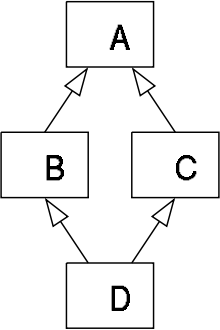
\includegraphics[scale=0.5]{files/diamond.png}}
\label{fig:diamond}
\caption{The diamond problem illustrated (source: Wikipedia)}
\end{figure}

A common multiple inheritance problem is the \textit{diamond problem}. This problem occurs when a class D inherits from classes B and C that have a common parent A. If D calls a method defined in A that has different behaviour in B and C then which version of the method will be called? C++ solves this problem by keeping a separate instance of A for both B and C, explicit qualification ensures that the correct version of the method is called. If B and C inherit A \textit{virtually}, then the compiler ensures that only one A object is constructed.

A C++ class does not inherit access rights in the same way that Objective-C does. The access right of the inherited class has to be explicitly mentioned. This access right then transfers to the members of that superclass. If the inherited class is declared public, then the access rights remain the same. If the inherited class is declared protected, then every public member of the superclass is protected in the subclass. If the inherited class is declared private, then every member of the superclass is private in the subclass.

\subsection{Constructors and Destructors}
\label{sec:constructor}
C++ constructors are normal methods with no return type and the class name as their signature. Method overloading (see section \ref{sec:overloading}) allows the definition of multiple constructors. Destructors in C++ are declared in a similar way, however, a destructor cannot accept any arguments and is named "\textit{\mytilde{}Classname()}". A destructor will be automatically called right before deleting an object.

The Objective-C language has no mandatory constructors or destructors. Constructing and deconstructing an object generally happens by overriding a few methods inherited from NSObject. These methods are listed here: 
\begin{itemize}
\item \textbf {alloc} Alloc allocates the space that the object needs.
\item \textbf {init} Init initialises the necessary instance variables.
\item \textbf {dealloc} Dealloc releases all the instance variables.
\end{itemize}

Note that nothing prevents an Objective-C programmer from creating his own alloc, init or dealloc that don't derive from NSObject directly or indirectly. For instance, a programmer that wants to implement the singleton pattern generally overrides alloc to ensure that an object is only created when he wants it.
Initialisers generally derive from NSObject's init at some point (via a call to super init). Conventions dictate that initialiser names start with init. Multiple initialisers are simply constructed by creating different methods, note that - unlike in C++, where a constructor has no return type or statement - an initialiser should return itself after instantiating the necessary instance variables.

\section{Language-Specific \-Features}
\subsection{Objective-C}
\subsubsection{Protocols}
\label{sec:protocol}
An Objective-C protocol defines a standard for objects to message each other. A protocol is simply a list of required and optional methods. A class 'A' that implements a protocol agrees to implement every required method of the protocol. A method or other class now knows that A will respond to the messages declared in the protocol. Reflection also allows other classes to see if a given class implements a certain protocol. An example of the use of protocols can be found in listing \ref{oc:pro}. Protocols allow us to work with objects without knowing the class of these objects, this allows a higher level of polymorphism, since we can ensure that the object we are working with will respond to a set of messages.

C++ has no protocol or interface keyword that allows us to declare a set of methods. It is possible to create interfaces in C++ by creating a class that only contains \textit{pure virtual} functions. A class that derives from this interface class can only be instantiated if it implements every pure virtual function that the interface declares. Section \ref{sec:abstract} expands on virtual functions in greater detail.

\subsubsection{Categories}
\label{sec:categories}
Objective-C categories were based on smalltalk categories and were introduced to make it easier to break classes down into smaller pieces. A category adds a set of methods to a class, these methods are added to the class at runtime. A category that extends a class can access all of the instance variables of this class, it's important to remember that a category is a class extension rather then an actual subclass. A category also has the ability to override existing methods of the class it extends.

Categories are generally used to either split the interface of a class over multiple files, or to extend pre-existing classes at runtime. Indeed, a category allows us to extend any class, regardless of where it's interface is located. This allows us to expand native and user-defined class on the fly.

C++ has no category system, and does not allow this amount of runtime flexibility. A C++ class cannot be changed at runtime. It's also impossible to split a class declaration over multiple header files. It is possible to split the class implementation. 

\subsubsection{Message Forwarding}
\label{sec:message}
Objective-C works with explicit message sending to objects. When an object receives a message, it looks up the method in the dispatch table of this object's class, If this is message is not recognised, then the message is looked up inside the superclass. An exception is thrown if the message is not recognised by the class highest in the hierarchy (NSObject).

Objective-C allows a programmer to intercept this process before the exception is thrown. The object receives the message  and has the ability to do as it pleases. This allows the programmer to use the message and to pas it along to another class. This feature is known as message forwarding. An example of message forwarding is presented in listing \ref{oc:for}. In this example an instance of A sends messages it does not understand to an instance of the B class if B can respond to this message. When we send the message doSomething to an instance of A, it will forward it to an instance of B, which can respond to this message. Message forwarding is often used when creating proxy objects.

Message forwarding can be used to mimic multiple inheritance in Objective-C (we can say that A inherits the doSomething method from B), it is important to realise that message forwarding is not a replacement for multiple inheritance though. Multiple inheritance adds features from different classes to a single class, while message forwarding divides responsibilities between different classes.

C++ does not offer message forwarding in the way the Objective-C does. It is possible to explicitly forward certain messages, but it is not possible to have a generic method that forwards every message it does not understand to another class. This is due to the fact that the C++ compiler returns errors when we call messages on an object that does not define them. In fact, sending a message to a C++ object is almost completely transformed into a method call by the compiler. This is another example of C++ favouring run-time efficiency over run-time flexibility.

\subsubsection{Reflection}
\label{sec:reflection}
Another example of the run-time flexibility of Objective-C is reflection. Reflection is the ability to examine and modify the behaviour of an object at runtime.

A listing of some of the reflective features of Objective-C is mentioned here. Keep in mind that this is only a listing of some basic features, the full list can be found at \cite{OCrefl}.
\begin{itemize}
\item Query an object about it's instance variables, type, superclass, protocols it implements or method list.
\item Get and Set instance variables
\item Add methods, replace methods
\end{itemize}

An example of adding and replacing methods is added in listing \ref{oc:ref}.

C++ has no reflection, by now this should come as no surprise, reflection happens purely at run-time and does not really fit in the run-time efficiency philosophy of C++.

\subsubsection{Metaclasses}
\label{sec:meta}
A lot of the inspiration for Objective-C came from smalltalk; in smalltalk, everything is an object, even classes are objects. The class of a class object is called the meta class. Meta classes also exist in Objective-C.

Objective-C classes have 2 different types of methods, instance methods are methods that work on a single instance, and class methods, methods that work on the class instance (which is an instance of the metaclass). These class methods don't require an initialised instance of class, and can be compared to static class methods in other languages. Class methods are simply instance methods of the meta-class. An example of a class method is alloc.

Metaclasses are also instances of a class, a metaclass is an instance of the NSObject metaclass. This means that every object has a parent class that is also an object, except for the metaclass of NSObject, the metaclass of NSObject is simply an instance of itself, this is the only class that is allowed to do this.

Metaclasses also have their own inheritance hierarchy, if class A inherits from class B, then metaclass A inherits from metaclass B. An illustration of all this can be found in figure \ref{fig:meta}.

C++ has no metaclasses.

\begin{figure}[h]
\centerline{
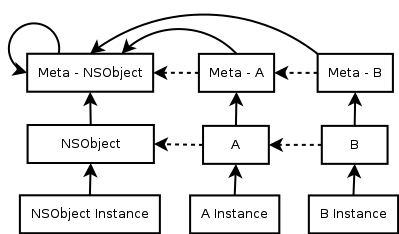
\includegraphics[scale=0.5]{files/meta.png}}
\caption{Inheritance and instance relations in Objective-C. A dashed line indicates an inheritance relation, while a normal line indicates an instance of relation.}
\label{fig:meta}
\end{figure}

\subsection{C++}
\subsubsection{Method Overloading}
\label{sec:overloading}
C++ allows the use of method overloading. This means that it is possible to create different methods with the same name, as long as their arity or argument types differ. Method overloading also works on constructors in C++.

Objective-C does not allow method overloading. This is generally not an issue due to the smalltalk-style messages that Objective-C uses (e.g. doSomethingWith A: (int) a andB: (int) b) which automatically differ when the arity of the method differs. The lack of method overloading is only an issue in Objective-C when we want to declare 2 functions with the same name, the same arity, but different variable types. We can use the id types as the type of the variable in combination with a double dispatch or a type-check as a substitute if having the same name is absolutely required.

\subsubsection{Namespaces}
\label{sec:namespaces}
Namespaces allow C++ programmers to divide their classes and other code into separate blocks. Data in a namespace is impossible to access without either prefixing it with \textit{namespacename::} or by adding "\textit{using namespace namespacename}" to the code. An example of namespaces is presented in listing \ref{cp:nam}.

This mechanism is especially useful when working on large code-bases, or when 3rd party libraries are used.

Objective-C has no similar mechanism for code separation. Convention dictates that classnames should have a 2 letter prefix that indicates the company or the product that this class belongs to. Examples of this are the NSString, NSArray, UIButton and various other classes. However, this convention only makes the problem less frequent rather then solving it. 

\subsubsection{Abstract Classes}
\label{sec:abstract}
An abstract class in C++ is a class that contains at least one pure virtual function. An abstract class cannot be instantiated on it's own. A class that derives from an abstract class without implementing every pure virtual function is also an abstract class. Abstract classes can be used for a number of things. One example that we presented earlier was the use of abstract classes to implement protocols (section \ref{sec:protocol}). Abstract classes are generally used to force a subclass to implement a certain method which can then be called in a polymorphic way.

Objective-C has no virtual keyword, since every method is virtual by default. Due to this, Objective-C has no abstract classes. We can however replace the pure virtual method of our C++ example by a method that simply throws an exception when it's called. This will raise an error at runtime if the "virtual" method is called by the abstract class.

\subsubsection{Friend Classes}
\label{sec:friend}
The friend class system allows a class to gain extra access rights to another class. If A declares B as it's friend, then B will receive access to all the methods and variables in A. It's important to note that this relation is not bidirectional, A will not gain access to the private variables that are part of B.

Objective-C doesn't have a friend system. We could replicate one by creating a category on A that provides all the extra functions that B needs. We can simply import this category into every class that needs friend access to A. This makeshift solution has it's drawbacks, any class can import this category, in the C++ system the friend is declared inside the class that gives access. In our solution, any class can just import the category and gain access into A, even if this is not intended. It's also possible to use reflection to access the private and protected members of A. Once more it is shown that access modifiers are checked at compile time and not at runtime.

\subsubsection{Inner Classes}
\label{sec:inner}

Inner classes are classes that are defined inside another class. The inner class can access the private, public and protected members of the outer class in C++. The outer class uses the standard rules when accessing the inner class.

Inner classes do not exist in Objective-C, it is possible to reach a similar effect by creating the inner class inside the implementation file of the outer class. This is just another class, but it's unreachable for other classes since it's never been declared inside any header file. The inner class will remain private to the implementation of the outer class, as long as the file that contains the interface of the inner class is never imported into another file.

\section{Conclusion}
Objective-C and C++ are both powerful object-oriented languages with a very different approach on adding objects to C. While C++ attempts to provide a language that is both close to the hardware and high level, with a focus on run-time efficiency and type safety at compile type; Objective-C tries to build a lightweight, smalltalk style object-oriented system on top of C that offers as much run-time flexibility as possible.

It's quite clear that both languages attract a different audience, even though they share a common ancestor. Both languages have their advantages that can drastically improve a project depending on the needs of the programmer.

%Bibliography
\printbibliography[heading = bibnumbered]

\section{Code Listings}
\lstinputlisting[label=cp:typ,language=C++,caption={Templates and static typing in C++}]{../C++/Types.cpp}
\lstinputlisting[label=oc:typ,caption={Objective-C using Dynamic and Static typing}]{../objC/Types.m}

\lstinputlisting[label=cp:acc,language=C++,caption={Access rights in C++}]{../C++/Access.cpp}
\lstinputlisting[label=oc:acc,caption={Access rights in Objective-C}]{../objC/Access.m}

\lstinputlisting[label=cp:pol,language=C++,caption={Polymorphism in C++}]{../C++/Polymorphism.cpp}
\lstinputlisting[label=oc:pol,caption={Polymorphism in Objective-C}]{../objC/Polymorphism.m}

\lstinputlisting[label=cp:inh,language=C++,caption={Inheritance in C++}]{../C++/Inheritance.cpp}
\lstinputlisting[label=cp:min,language=C++,caption={Multiple inheritance in C++}]{../C++/MultipleInheritance.cpp}
\lstinputlisting[label=oc:inh,caption={Inheritance in Objective-C}]{../objC/Inheritance.m}


\end{document}
